\documentclass[11pt,a4paper]{article}
\usepackage[utf8]{inputenc}
\usepackage[T1]{fontenc}
\usepackage{lmodern}
\usepackage[provide=*,spanish]{babel}
\usepackage[margin=2.2cm]{geometry}
\usepackage{booktabs,tabularx,array}
\usepackage{tikz}
\usetikzlibrary{positioning,arrows.meta,fit}
\usepackage{listings}
\usepackage{xcolor}
\usepackage{enumitem}
\usepackage{multirow}
\usepackage[hidelinks]{hyperref}

\setlist{itemsep=1pt,topsep=3pt}
\setlength{\parskip}{4pt}
\setlength{\parindent}{0pt}
\lstset{basicstyle=\ttfamily\small,columns=fixed,basewidth=0.5em,frame=single,
        framerule=0.3pt,rulecolor=\color{gray},backgroundcolor=\color{gray!6},
        xleftmargin=4pt,xrightmargin=4pt,aboveskip=6pt,belowskip=6pt}
\newcommand{\code}[1]{\texttt{#1}}
\newcolumntype{L}{>{\raggedright\arraybackslash}X}

\title{\textbf{Procesador RISC-V ERV26 con pipeline de 5 etapas}\\[2pt]
\large Proyecto \code{risvV\_E5} --- 25.30 Electrónica V (ITBA)}
\author{Matias Minniti \and Iñaqui Alonso \and Facundo Torres \and Rocco Gastaldi}
\date{Noviembre 2026}

\begin{document}
\maketitle

\section{Resumen}

ERV26 es un procesador RV32I con pipeline de 5 etapas (IF, ID, EX, MEM, WB) implementado en la placa DE10-Nano (Cyclone V 5CSEBA6U23I7). 

\begin{center}
\begin{tabular}{ll}
\toprule
ISA & RV32I (sin \code{FENCE.I}, CSR ni traps) \\
Pipeline & 5 etapas, forwarding completo, predicción BTFN, lectura anticipada \\
Memorias & 16\,KB programa + 16\,KB datos + framebuffer doble, en M10K \\
Periféricos & LEDs, switches, botones en GPIO, video HDMI 640$\times$480 \\
CPI medido & 1,06 (\code{arith.c}) y 1,09 (\code{sort\_crc.c}), también con la RAM de la placa \\
Recursos & 1\,784 ALMs de 41\,910 (4\,\%), 1\,645 registros, 192 bloques M10K de 553 (35\,\%) \\
Reloj & 50\,MHz en la placa; Fmax 64,96\,MHz en el peor caso (slack +4,607\,ns) \\
Verificación & 144/144 tests en 5 condiciones; 74/74 sobre el netlist post-fit \\
\bottomrule
\end{tabular}
\end{center}

\section{Arquitectura}

\subsection{Pipeline}

\begin{figure}[h]
\centering
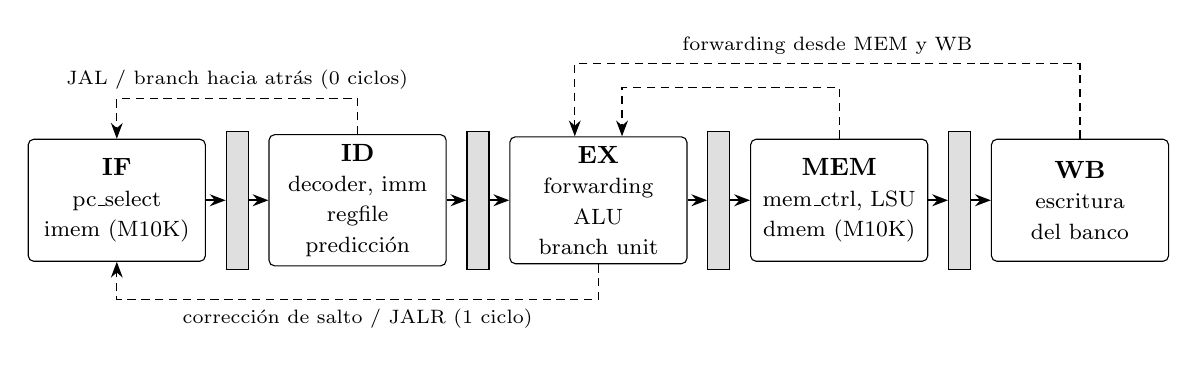
\begin{tikzpicture}[
  st/.style={draw,rounded corners=2pt,minimum width=2.25cm,minimum height=1.55cm,align=center,font=\small},
  lt/.style={draw,fill=gray!25,minimum width=0.28cm,minimum height=1.75cm},
  ar/.style={-{Stealth[length=2mm]},thick},
  fb/.style={-{Stealth[length=2mm]},densely dashed}]
\node[st] (if) {\textbf{IF}\\ \footnotesize pc\_select\\ \footnotesize imem (M10K)};
\node[lt,right=0.25cm of if] (l1) {};
\node[st,right=0.25cm of l1] (id) {\textbf{ID}\\ \footnotesize decoder, imm\\ \footnotesize regfile\\ \footnotesize predicción};
\node[lt,right=0.25cm of id] (l2) {};
\node[st,right=0.25cm of l2] (ex) {\textbf{EX}\\ \footnotesize forwarding\\ \footnotesize ALU\\ \footnotesize branch unit};
\node[lt,right=0.25cm of ex] (l3) {};
\node[st,right=0.25cm of l3] (mem) {\textbf{MEM}\\ \footnotesize mem\_ctrl, LSU\\ \footnotesize dmem (M10K)};
\node[lt,right=0.25cm of mem] (l4) {};
\node[st,right=0.25cm of l4] (wb) {\textbf{WB}\\ \footnotesize escritura\\ \footnotesize del banco};
\foreach \a/\b in {if/l1,l1/id,id/l2,l2/ex,ex/l3,l3/mem,mem/l4,l4/wb} \draw[ar] (\a) -- (\b);
\draw[fb] (id.north) -- ++(0,0.45) -| node[pos=0.25,above,font=\scriptsize]{JAL / branch hacia atrás (0 ciclos)} (if.north);
\draw[fb] (ex.south) -- ++(0,-0.45) -| node[pos=0.25,below,font=\scriptsize]{corrección de salto / JALR (1 ciclo)} (if.south);
\draw[fb] (mem.north) -- ++(0,0.65) -| ([xshift=3mm]ex.north);
\draw[fb] (wb.north) -- ++(0,0.95) -| node[pos=0.25,above,font=\scriptsize]{forwarding desde MEM y WB} ([xshift=-3mm]ex.north);
\end{tikzpicture}
\caption{Etapas del pipeline. En gris, los latches entre etapas.}
\end{figure}

Todas las etapas usan el mismo reloj de 50\,MHz; el avance se controla con señales de habilitación, sin relojes desfasados.

\textbf{Fetch sin ciclo extra.} La memoria de programa M10K tiene lectura sincrónica. Para no agregar una etapa, el núcleo le entrega la dirección de la \emph{próxima} instrucción (\code{imem\_addr}), la memoria la registra en el flanco y su salida es directamente la instrucción que está en ID.

\textbf{Hazards de datos.}
\begin{itemize}
\item \emph{Forwarding} desde EX/MEM y MEM/WB hacia EX, para ambos operandos y para el dato de los stores.
\item \emph{Bypass} WB$\to$ID dentro del banco de registros: un registro escrito en WB se lee actualizado en ID en el mismo ciclo.
\item \emph{Load-use}: si una instrucción usa el resultado de un load que está en EX, se detiene un ciclo y luego el dato llega por forwarding.
\end{itemize}

\textbf{Saltos: predicción estática BTFN} (\emph{backward taken, forward not taken}). El destino PC+imm no depende de registros, así que se calcula en ID.

\begin{center}
\begin{tabular}{llc}
\toprule
Caso & Predicción en ID & Ciclos perdidos \\
\midrule
JAL & siempre tomado & 0 \\
Branch hacia atrás (cierra loops) & tomado & 0 si acierta, 1 si no \\
Branch hacia adelante & no tomado & 0 si acierta, 1 si no \\
JALR & --- (depende de un registro) & 1 \\
Load seguido de uso & --- & 1 \\
\bottomrule
\end{tabular}
\end{center}

En código compilado, los loops cierran con un branch hacia atrás que casi siempre se toma. Frente a predecir siempre ``no tomado'', BTFN reduce los ciclos perdidos en saltos de 2\,105 a 1\,222 en \code{sort\_crc.c} ($-4{,}3\,\%$ de ciclos totales).

\textbf{Control del pipeline.} La unidad de hazards genera tres señales:
\begin{itemize}
\item \code{freeze} congela todo el pipeline. Se activa con \code{en}=0 (halt externo, botón KEY1) o mientras un acceso a memoria espera \code{memory\_ready}.
\item \code{load\_use} detiene PC e IF/ID e inserta una burbuja en ID/EX.
\item \code{flush\_id} descarta la instrucción en ID cuando EX corrige un salto.
\end{itemize}

\textbf{Memoria con \code{memory\_ready}.} El núcleo mantiene \code{req}, \code{addr}, \code{we}, \code{be} y \code{wdata} estables hasta recibir \code{ready}. Si la memoria responde mientras el pipeline está congelado por otro motivo, el acceso se marca como hecho y se guarda el dato leído. Así un store nunca se ejecuta dos veces, lo que importa con periféricos.

\textbf{Lectura anticipada de la memoria de datos.} La M10K registra la dirección en el flanco y entrega el dato en el ciclo siguiente. Si la dirección llegara recién con el load en MEM, cada load esperaría un ciclo. Por eso el núcleo da una salida extra, \code{dmem\_addr\_next}: la dirección que va a tener la instrucción de MEM en el ciclo siguiente. Es la del load que está en EX o, si el pipeline está congelado, la misma de MEM. La memoria lee esa dirección por adelantado y, cuando el load llega a MEM, el dato ya está listo. Es el mismo recurso que usa el fetch con la memoria de programa.

La memoria confirma \code{ready} solo si la dirección leída coincide con la del acceso y si esa lectura no chocó con una escritura a la misma palabra en el mismo flanco. En la M10K, leer y escribir la misma palabra a la vez da un valor indefinido; Quartus la infiere con \emph{read-during-write} ``don't care''. En ese caso, que solo ocurre cuando un load lee la palabra que el store anterior está escribiendo, la memoria tarda un ciclo más, pero nunca entrega un dato equivocado.

\textbf{Instrucciones no soportadas.} \code{FENCE} y las instrucciones SYSTEM (ECALL, EBREAK, CSR) se ejecutan como NOP. Las instrucciones ilegales también son NOP, y los accesos desalineados no generan trap.

\subsection{Mapa de memoria}

Arquitectura Harvard con un único espacio de direcciones. \code{.rodata} va a la memoria de datos para que los loads puedan leerla.

\begin{center}
\begin{tabular}{lll}
\toprule
Dirección & Contenido & Acceso \\
\midrule
\code{0x0000\_0000} & memoria de programa, 16\,KB (\code{.text}) & fetch \\
\code{0x0001\_0000} & memoria de datos, 16\,KB (datos, \code{.bss} y pila) & R/W \\
\code{0x8000\_0000} & LEDs (8 bits) & R/W \\
\code{0x8000\_0004} & switches (4 bits) & R \\
\code{0x8000\_0008} & contador de ciclos (32 bits, 50\,MHz) & R \\
\code{0x8000\_000C} & botones (GPIO\_0[3:0], 1 = apretado) & R \\
\code{0x8000\_0010} & contador de cuadros de video (60\,Hz) & R \\
\code{0x8000\_0014} & página del framebuffer que se muestra & R/W \\
\code{0x4000\_0000} & framebuffer: 2 páginas de 320$\times$240, RGB332 & W \\
\bottomrule
\end{tabular}
\end{center}

La E/S se mapea en memoria en lugar de atar los registros x28--x31 a puertos, porque gcc usa esos registros (t3--t6) libremente.

\section{Bloques}

\subsection{Top de la placa (\code{risvV\_E5.bdf})}

\begin{center}
\begin{tabularx}{\linewidth}{lL}
\toprule
Bloque & Función \\
\midrule
\code{erv26\_board\_ctrl} & Sincroniza el reset (KEY0, asincrónico al presionar y sincrónico al soltar) y el halt (KEY1 mantenido $\Rightarrow$ \code{en}=0). \\
\code{erv26\_core} & Núcleo con pipeline (diagrama \code{rtl/erv26\_core.bdf}, ver abajo). \\
\code{erv26\_imem} & Memoria de programa M10K de 16\,KB, inicializada con \code{imem.hex}. \\
\code{erv26\_bus} & Decodifica el bus de datos: E/S si \code{addr[31]}=1, framebuffer si \code{addr[31:30]}=01, RAM en otro caso. Reparte \code{req} y multiplexa \code{rdata}/\code{ready}. \\
\code{erv26\_dmem} & Memoria de datos M10K \emph{simple dual-port} de 16\,KB, en 4 bancos de 8 bits (uno por byte enable), inicializada con \code{dmem\_b0..3.hex}. Lee por adelantado la dirección \code{addr\_next} que le da el núcleo, así que escrituras y lecturas se completan sin espera. \\
\code{erv26\_io} & LEDs, switches y botones (sincronizados), contador de ciclos, contador de cuadros y página de video; responde en el mismo ciclo. \\
\code{erv26\_video} & Framebuffer doble en M10K y generador de video 640$\times$480 a 60\,Hz para el ADV7513. \\
\code{erv26\_hdmi\_init} & Configura el transmisor HDMI ADV7513 por I2C, y repite la configuración cada $\sim$0,7\,s. \\
\bottomrule
\end{tabularx}
\end{center}

\subsection{Núcleo (\code{rtl/erv26\_core.bdf})}

\begin{center}
\small
\begin{tabularx}{\linewidth}{llL}
\toprule
Etapa & Bloque & Función \\
\midrule
IF & \code{pc\_select} & Próxima dirección de fetch, por prioridad: freeze $\to$ corrección de EX $\to$ load-use $\to$ salto desde ID $\to$ PC+4. \\
   & \code{if\_id} & Latch IF/ID: PC de la instrucción en ID y bit de validez. \\
\midrule
ID & \code{decoder} & Separa los campos de la instrucción y genera las señales de control. \\
   & \code{imm\_gen} & Inmediato con extensión de signo según el formato (I/S/B/U/J). \\
   & \code{regfile} & 31 registros + x0; dos lecturas asincrónicas y bypass de la escritura de WB. \\
   & \code{id\_predict} & Destino PC+imm; redirige el fetch en los JAL y en los branches hacia atrás, y marca \code{pred\_taken}. \\
   & \code{hazard\_unit} & Genera \code{freeze}, \code{load\_use} y \code{flush\_id}. \\
\midrule
ID/EX & \code{id\_ex} & Latch con operandos, inmediato y control; inserta burbujas por load-use o flush. \\
\midrule
EX & \code{forward\_unit} & Elige para cada operando el valor más nuevo: EX/MEM, MEM/WB o el banco. \\
   & \code{operand\_build} & Operando A (rs1/PC/0) y B (rs2/inmediato) de la ALU. \\
   & \code{alu} & ADD, SUB, SLL, SLT, SLTU, XOR, SRL, SRA, OR, AND. \\
   & \code{branch\_unit} & Comparador y sumadores propios. Resuelve el salto, lo compara con la predicción y corrige si hace falta. \\
   & \code{ex\_result} & Resultado de la etapa: salida de la ALU o PC+4 (link de JAL/JALR). \\
\midrule
EX/MEM & \code{ex\_mem} & Latch con resultado, dato a guardar y control de memoria. \\
\midrule
MEM & \code{mem\_ctrl} & Handshake \code{req}/\code{ready}; evita repetir un acceso que ya se hizo y genera la dirección de lectura anticipada (\code{dmem\_addr\_next}). \\
    & \code{lsu} & Stores: byte enables y replicación del dato (SB/SH/SW). Loads: selección de byte/halfword y extensión de signo. \\
    & \code{wb\_select} & Dato a escribir: el del load o el resultado de EX. \\
\midrule
MEM/WB & \code{mem\_wb} & Latch con el dato de write-back. \\
\midrule
WB & \code{wb\_commit} & Habilita la escritura del banco de registros y genera las salidas de debug (\code{dbg\_commit\_*}) que usa la verificación. \\
\bottomrule
\end{tabularx}
\end{center}

\section{Video HDMI y programa cargado}

\subsection{Video}

\code{erv26\_video} genera la imagen de 640$\times$480 a 60\,Hz (timing VESA, píxel de 25\,MHz). Para no cruzar dominios de reloj, trabaja con el mismo reloj de 50\,MHz que el procesador y avanza un píxel cada dos ciclos. El framebuffer tiene dos páginas de 320$\times$240 píxeles a un byte por píxel (RGB332), y cada píxel se muestra como un bloque de 2$\times$2. El procesador dibuja en una página mientras se ve la otra y después pide el cambio. El cambio se aplica al empezar el blanking vertical, así que nunca se ve una imagen a medio dibujar. \code{erv26\_hdmi\_init} escribe por I2C los registros del ADV7513 que indica su guía de programación: encendido, registros fijos y formato RGB 4:4:4 de 24 bits.

\subsection{Invasores del espacio}

El \code{.sof} trae cargado \code{sw/games/invaders/invaders.c}, un juego estilo arcade escrito en C para el ERV26, con gráficos y fuente propios. Tiene 5 filas de 11 invasores que aceleran a medida que caen, 4 escudos destructibles, un platillo misterioso, oleadas sucesivas, puntaje, récord y 3 vidas (que se ven en los LEDs). Cada cuadro, el programa lee los botones, actualiza el juego, redibuja la página oculta y espera al siguiente blanking. Usa $\sim$17\,\% del tiempo del cuadro, así que siempre va a 60\,fps.

\begin{center}
\begin{tabular}{llll}
\toprule
Pin de JP1 & Señal & Botón & Conexión \\
\midrule
1 & \code{GPIO\_0[0]} & izquierda & \multirow{4}{*}{entre el pin y GND (JP1 pin 12 o 30)} \\
2 & \code{GPIO\_0[1]} & derecha & \\
3 & \code{GPIO\_0[2]} & disparo & \\
4 & \code{GPIO\_0[3]} & start & \\
\bottomrule
\end{tabular}
\end{center}

Las entradas tienen pull-up interno, así que basta un pulsador entre cada pin y GND. KEY0 sigue siendo reset y KEY1, halt. La demo de LEDs anterior (\code{sw/demo/leds.c}) se puede volver a cargar con \code{build.py}.

\section{Verificación}

\subsection{Método}

Cada programa de prueba se ejecuta en dos lugares:
\begin{enumerate}
\item En un \emph{modelo de referencia} (ISS, \code{tools/erv26\_iss.py}): un simulador de RV32I escrito aparte, que decodifica las instrucciones de forma independiente del hardware.
\item En el núcleo, simulado con Icarus Verilog (\code{sim/tb\_core.v}). La regresión convierte primero \code{erv26\_core.bdf} a Verilog con \code{tools/bdf2v.py}, así que se simula el mismo diagrama que sintetiza Quartus.
\end{enumerate}
Se compara \emph{instrucción por instrucción} la secuencia de instrucciones retiradas: PC, instrucción, registro destino y valor escrito. También se compara la secuencia completa de stores. Además, el testbench tiene \emph{asserts} internos: dependencia de un load sin stall, X en el PC o X en un write-back.

Cada programa corre en cinco condiciones de memoria y halt. Las tres primeras usan un modelo de memoria con latencia aleatoria, que prueba que el núcleo funciona con cualquier memoria que respete el protocolo. Las dos últimas usan la RAM real de la placa (\code{erv26\_dmem}). Mientras la memoria no responde, el testbench le entrega basura al núcleo, así que usar un dato antes de \code{ready} se detecta. Con la RAM real, si la M10K leyó y escribió la misma palabra en el mismo flanco, el testbench reemplaza su dato por \code{DEADBEEF}, así que usar ese valor indefinido también se detecta.

\begin{center}
\begin{tabular}{lll}
\toprule
Condición & \code{memory\_ready} & \code{en} (halt) \\
\midrule
\code{lat0} & siempre listo & siempre 1 \\
\code{lat3} & latencia aleatoria de 0 a 3 ciclos & siempre 1 \\
\code{lat2+halt} & latencia aleatoria de 0 a 2 ciclos & aleatorio \\
\code{m10k} & RAM de la placa (M10K, lectura anticipada) & siempre 1 \\
\code{m10k+halt} & RAM de la placa & aleatorio \\
\bottomrule
\end{tabular}
\end{center}

\subsection{Suites y resultados}

\begin{center}
\begin{tabularx}{\linewidth}{lLc}
\toprule
Suite & Contenido & Resultado \\
\midrule
riscv-tests \code{rv32ui} & 40 tests oficiales de RV32I, incluidos los de bypass con 0, 1 y 2 instrucciones intermedias. No se corren \code{fence\_i} ni \code{ma\_data}, que prueban funciones no implementadas. & 40/40 \\
C & quicksort, CRC32, recursión, punteros a función, mul/div por software y accesos de 8/16 bits. & 2/2 \\
Dirigidos (asm) & \code{branch\_pred.S}: 8 casos borde de la predicción (load justo antes de un branch hacia atrás, JALR tras una predicción fallida, loops anidados). \code{mem\_access.S}: 8 casos de acceso a memoria (store seguido de load a la misma palabra, punteros encadenados, copias solapadas). & 2/2 \\
Aleatorios & Programas generados con branches, loops, JAL/JALR, loads/stores y dependencias densas. & 100/100 (+500) \\
MVP-0 & Regresión del procesador single-cycle (checkpoint 1). & 51/51 \\
\bottomrule
\end{tabularx}
\end{center}

Para comprobar que la regresión detecta errores, se inyectaron bugs a propósito, uno por vez. En una etapa anterior del proyecto fueron 8 bugs típicos de pipeline (sin forwarding, sin stall load-use, sin flush, doble acceso a memoria, etc.), y todos fueron detectados. Para la lectura anticipada se probaron 3 más:
\begin{itemize}
\item \code{ready} sin chequear el choque entre lectura y escritura: \code{mem\_access} falla porque lee \code{DEADBEEF}.
\item Dirección anticipada sin tener en cuenta \code{freeze}: \code{mem\_access} falla por timeout.
\item Sin lectura anticipada: los tests pasan, pero con la RAM real el programa tarda un 8,6\,\% más. Así se mide la mejora.
\end{itemize}

\subsection{Placa completa y netlist de Quartus}

\begin{itemize}
\item \textbf{Top de placa:} se simulan los dos \code{.bdf} anidados con las memorias, el bus y la E/S reales. Pasan la demo de LEDs (\code{tb\_board.v}) y los programas \code{sort\_crc}, \code{arith}, \code{branch\_pred} y \code{mem\_access}, que informan el resultado en los LEDs. Tardan lo mismo que el núcleo con memoria ideal, más 2 ciclos de salida del reset.
\item \textbf{Gate-level:} el proyecto auxiliar \code{gate\_sim/core\_gl.qpf} compila solo el núcleo y exporta el netlist post-fit (\code{.vo}). La regresión corre sobre ese netlist con los modelos de celdas del Cyclone V (\lstinline{--gate}). Así se comprueba que Quartus interpretó bien los diagramas y el Verilog. Con la versión actual (predicción BTFN y lectura anticipada) pasaron 74/74 tests en las 5 condiciones (40 riscv-tests, 2 en C, 2 dirigidos y 30 aleatorios), con los mismos ciclos que el RTL.
\item \textbf{Video:} \code{sim/video/tb\_video.v} llena las dos páginas con patrones, captura dos cuadros de la salida HDMI y los compara píxel a píxel con lo esperado. También mide el timing: 800$\times$525 píxeles, sincronismos de 96 píxeles y de 2 líneas, y 640$\times$480 activos. \code{tb\_i2c.v} decodifica el bus I2C y lista las escrituras al ADV7513.
\item \textbf{Juego:} se simula la placa completa corriendo el juego, con los botones manejados por el testbench (\code{tb\_game.v}). La imagen HDMI que genera el ERV26 coincide píxel a píxel con la que produce el mismo código compilado para la PC.
\item \textbf{Timing:} lo verifica el Timing Analyzer de Quartus, porque el netlist de Cyclone V es funcional y no tiene retardos.
\end{itemize}

\subsection{Cómo correrla}

\begin{lstlisting}
cd sim
python3 run_core_tests.py -j 2                    # regresion completa
python3 run_core_tests.py --suite random --random 500
python3 run_core_tests.py --only rv32ui-lw --vcd  # un test, con formas de onda
\end{lstlisting}

{\sloppy Requisitos: Python 3, Icarus Verilog, el toolchain
\code{riscv64-unknown-elf-gcc} y el repositorio \code{riscv-tests} clonado al lado del proyecto.\par}

\section{Compilar y cargar otro programa}

\subsection{Escribir el programa}

Los programas se escriben en C (o assembler) sin sistema operativo ni biblioteca estándar. Para la E/S se incluye \code{sw/common/erv26.h}:

\noindent\begin{minipage}{\linewidth}
\begin{lstlisting}[language=C]
#include "erv26.h"
int main(void) {
    for (;;) LEDS = SWITCHES;      /* LEDs = estado de los switches */
}
\end{lstlisting}
\end{minipage}

El arranque (\code{sw/common/crt0.S}) inicializa \code{sp} y \code{gp}, limpia \code{.bss} y llama a \code{main}. El linker script (\code{link.ld}) ubica el código en la memoria de programa y los datos en la de datos. Al no haber multiplicador en hardware, gcc resuelve \code{*}, \code{/} y \code{\%} con rutinas de \code{libgcc}.

\subsection{Compilar}

\begin{lstlisting}
python3 sw/build.py mi_programa.c
\end{lstlisting}

Para el juego hay que agregar su carpeta con \code{-I}:
\begin{lstlisting}
python3 sw/build.py sw/games/invaders/invaders.c -I sw/games/invaders
\end{lstlisting}

\code{build.py} compila con \code{-march=rv32i -mabi=ilp32 -O2} y convierte el ELF a archivos de inicialización. Los deja en la raíz del proyecto, que es donde los lee Quartus:

\begin{center}
\begin{tabular}{ll}
\toprule
Archivo & Uso \\
\midrule
\code{imem.hex} & contenido de la memoria de programa \\
\code{dmem\_b0..3.hex} & contenido inicial de la memoria de datos, un archivo por byte \\
\code{prog.lst} & desensamblado, útil para depurar \\
\code{prog.elf}, \code{imem.mif}, \code{dmem.hex} & ejecutable y formatos alternativos \\
\bottomrule
\end{tabular}
\end{center}

\subsection{Cargar en la placa}

\begin{enumerate}
\item En Quartus, abrir \code{risvV\_E5.qpf} y compilar (\emph{Processing} $\to$ \emph{Start Compilation}). Hace falta recompilar porque el programa queda grabado en el \code{.sof} como contenido inicial de las M10K.
\item Conectar el USB-Blaster II de la DE10-Nano y abrir \emph{Tools} $\to$ \emph{Programmer}. En \emph{Hardware Setup} elegir \code{DE-SoC} y hacer \emph{Auto Detect}.
\item Sobre el dispositivo \code{5CSEBA6} (no el HPS), elegir \emph{Change File} $\to$ \code{output\_files/risvV\_E5.sof}, tildar \emph{Program/Configure} y presionar \emph{Start}.
\end{enumerate}

La configuración es volátil: al cortar la alimentación hay que volver a programar.

\subsection{Probar antes en simulación}

Un programa que termine (\code{main} retorna 0) se puede comparar contra el ISS copiándolo a \code{sw/tests/} y corriendo \lstinline{python3 run_core_tests.py --suite c}. Al terminar, \code{crt0.S} escribe el resultado en \code{TOHOST} y la simulación termina.

\section{Rendimiento}

\begin{center}
\begin{tabular}{lrrccc}
\toprule
 & & & \multicolumn{3}{c}{CPI} \\
\cmidrule(lr){4-6}
Programa & Instrucciones & Ciclos & actual & sin BTFN & sin lectura anticipada \\
\midrule
\code{arith.c} & 18\,157 & 19\,275 & 1,06 & 1,08 & 1,16 \\
\code{sort\_crc.c} & 17\,851 & 19\,467 & 1,09 & 1,14 & 1,19 \\
\bottomrule
\end{tabular}
\end{center}

Los ciclos son los mismos con la memoria ideal de la simulación y con la RAM real de la placa. Los que se pierden vienen de saltos mal predichos o JALR y de los stalls por load-use (1 ciclo cada uno). La última columna muestra el CPI con la RAM de la placa si no hubiera lectura anticipada: cada load esperaría un ciclo.

\section{Implementación en la FPGA}

Resultados de Quartus Prime 25.1 Lite para la placa completa (núcleo, memorias, bus, E/S, video e I2C) en el Cyclone V 5CSEBA6U23I7.

\subsection{Frecuencia máxima}

{\sloppy El único reloj es el oscilador de 50\,MHz de la placa (\code{FPGA\_CLK1\_50}), restringido a 20\,ns en \code{risvV\_E5.sdc}. El Timing Analyzer analiza los cuatro modelos de la FPGA (proceso lento y rápido, a $-40$ y 100\,\textdegree C):\par}

\begin{center}
\begin{tabular}{lccc}
\toprule
Modelo & Fmax & Slack de setup a 50\,MHz & Slack de hold \\
\midrule
Lento, 1100\,mV, 100\,\textdegree C & 65,32\,MHz & +4,690\,ns & +0,274\,ns \\
Lento, 1100\,mV, $-40$\,\textdegree C & \textbf{64,96\,MHz} & \textbf{+4,607\,ns} & +0,261\,ns \\
Rápido, 1100\,mV, 100\,\textdegree C & --- & +11,704\,ns & +0,138\,ns \\
Rápido, 1100\,mV, $-40$\,\textdegree C & --- & +13,024\,ns & \textbf{+0,121\,ns} \\
\bottomrule
\end{tabular}
\end{center}

La frecuencia máxima en el peor caso es \textbf{64,96\,MHz}: el camino más largo tarda $20 - 4{,}607 = 15{,}39$\,ns. El diseño corre a 50\,MHz con un 23\,\% de margen, y todos los slacks son positivos. El \code{.sdc} también restringe los pines de E/S, así que no quedan caminos sin analizar. Los botones, switches e I2C son asincrónicos o lentos y pasan por sincronizadores. Las salidas de video salen de registros en las celdas de E/S y el dato queda estable 20\,ns antes del flanco de \code{HDMI\_TX\_CLK}.

Los caminos más largos son los de redireccionamiento del PC, que en un mismo ciclo van de una M10K a la dirección de otra:
\begin{itemize}
\item salida de la memoria de programa $\to$ decodificación y sumador de JAL/predicción en ID $\to$ dirección de la memoria de programa;
\item forwarding $\to$ ALU o comparador de branches en EX $\to$ dirección de la memoria de programa o de la lectura anticipada de datos.
\end{itemize}
Subir el reloj por encima de 50\,MHz requeriría un PLL y adaptar el generador de video, que hoy obtiene el píxel de 25\,MHz dividiendo por dos el mismo reloj.

\subsection{Recursos utilizados}

\begin{center}
\begin{tabular}{lrrr}
\toprule
Recurso & Usado & Disponible & \% \\
\midrule
Lógica (ALMs) & 1\,784 & 41\,910 & 4\,\% \\
Registros & 1\,645 & --- & --- \\
Bloques de memoria M10K & 192 & 553 & 35\,\% \\
Bits de memoria & 1\,490\,944 & 5\,662\,720 & 26\,\% \\
Pines & 49 & 314 & 16\,\% \\
Bloques DSP & 0 & 112 & 0\,\% \\
PLLs & 0 & 6 & 0\,\% \\
\bottomrule
\end{tabular}
\end{center}

De los 1\,645 registros, 1\,617 son de lógica y 28 están en las celdas de E/S de la salida de video. No se usan DSP porque RV32I no tiene multiplicación.

\textbf{Por bloque.} Datos del reporte \emph{Resource Utilization by Entity} del Fitter:

\begin{center}
\begin{tabular}{lrrr}
\toprule
Bloque & ALMs & Registros & M10K \\
\midrule
\code{erv26\_core} (núcleo) & 1\,543 & 1\,389 & 0 \\
\quad \code{regfile} (banco de registros) & 659 & 997 & 0 \\
\quad \code{alu} & 210 & 0 & 0 \\
\quad \code{id\_ex} (latch ID/EX) & 65 & 180 & 0 \\
\quad \code{ex\_result} & 142 & 0 & 0 \\
\quad \code{branch\_unit} & 85 & 0 & 0 \\
\quad \code{forward\_unit} & 77 & 0 & 0 \\
\quad \code{operand\_build} & 73 & 0 & 0 \\
\quad \code{pc\_select} & 63 & 0 & 0 \\
\quad resto del núcleo (latches, decoder, MEM, etc.) & 169 & 212 & 0 \\
\code{erv26\_video} (framebuffer y generador) & 103 & 47 & 160 \\
\code{erv26\_hdmi\_init} (I2C) & 57 & 61 & 0 \\
\code{erv26\_io} & 41 & 103 & 0 \\
\code{erv26\_bus} & 20 & 0 & 0 \\
\code{erv26\_dmem} (memoria de datos) & 18 & 13 & 16 \\
\code{erv26\_imem} (memoria de programa) & 0 & 0 & 16 \\
\code{erv26\_board\_ctrl} & 1 & 4 & 0 \\
\midrule
Total & 1\,784 & 1\,617 & 192 \\
\bottomrule
\end{tabular}
\end{center}

El banco de registros ocupa casi la mitad de la lógica del núcleo. Se implementa con flip-flops (31$\times$32 = 992 bits más el control), no en M10K. Necesita dos lecturas asincrónicas en el mismo ciclo y el bypass de la escritura de WB, y las M10K solo leen de forma sincrónica.

\textbf{Bloques de memoria.} Cada M10K tiene 10\,240 bits:

\begin{center}
\begin{tabularx}{\linewidth}{lrrL}
\toprule
Memoria & Bits & M10K & Organización \\
\midrule
Programa (\code{erv26\_imem}) & 131\,072 & 16 & 4\,096 palabras de 32 bits \\
Datos (\code{erv26\_dmem}) & 131\,072 & 16 & 4 bancos de 4\,096$\times$8 bits (uno por byte) \\
Video (\code{erv26\_video}) & 1\,228\,800 & 160 & 2 páginas de 320$\times$240 bytes, en 4 bancos de 38\,400$\times$8 \\
\midrule
Total & 1\,490\,944 & 192 & \\
\bottomrule
\end{tabularx}
\end{center}

El framebuffer ocupa el 83\,\% de los bloques de memoria usados. Aun así quedan 361 M10K libres (65\,\%), suficientes para agrandar la memoria de programa o de datos.

\end{document}
